\subsection{Power Electronics}

\subsubsection{Theory}
%Introduce the required theory that underlines the analysis for selection of each component.
For successful flight of the proposed prototype, power electronics are required to integrate control and provide propulsion. As discussed in literature, key components include a flight controller, BLDC motors, ESCs, servo motors, a Lipo battery, data telemetry, control links and camera sensors (REF HERE). Furthermore, depending on the complexity of the mission profile, an auxiliary companion computer is required to support high level autonomy and control \cite{deci1995human}.\\

Due to CASA regulations, a drone piloted under no certification can not exceed two kilograms in total flight weight \cite{CASA}. As a result, power electronics for propulsion and mechanical control will be sized to meet this regulation. Although the final manufactured prototype will exceed this weight category, a preliminary minimum complexity VTOL system will be sized and constructed allowing power electronics integration techniques to be verified.\\

Of all power electronics discussed, those imperative for a minimum complexity controlled VTOL system include BLDC motors and corresponding propellers, ESCs, servo motors, a Lipo battery, control link and flight controller \cite{vervoorst2016modular}.\\

When considering BLDC motor sizing, the KV rating is imperative to consider. The KV rating of a motor describes the increase in RPM per one volt increase in the supplied voltage with no load on the motor \cite{shaikh2017design}. KV rating and torque produced by the motor are inversely proportional, hence a lower KV rated motor coupled with a larger propeller will produce higher torque \cite{shaikh2017design}.\\

For effective BLDC motor control, ESC selection is of high importance. The ESC module governs the voltage sent to the BLDC motor \cite{green2015modeling}. Through a PWM control signal sent from the flight controller, the ESC manipulates the duty cycle and frequency of the three phase voltage waveform, adjusting the motors speed and torque as required \cite{green2015modeling}. Commercially available ESCs come in a variety of maximum amperage sizes and corresponding switching frequencies and internal resistance \cite{green2015modeling}. Sizing of this module is performed once a BLDC motor is selected which governs the voltage required, hence maximum amperage requirement for the ESC module.\\

For precise control of mechanical systems such as the tilt-wing mechanism, voltage feedback servo motors provide sufficient capabilities. Through PWM signals generated from the flight controller, servo position can be precisely adjusted with a PID feedback loops. \cite{van1981motor}. When selecting servo motors for a specific application, variables such as torque to inertia ratio, speed range and peak torque are imperative to consider \cite{krishnan1987selection}. In this section, an arbitrary servo motor will be selected given the minimum complexity controlled VTOL system will not represent the forces experienced by mechanism in the final prototype.\\

As discussed in previous literature, Lipo batteries provide the highest energy density, thus are most suitable for electric VTOL systems (REF HERE). After a BLDC motor is selected, with corresponding voltage requirements, a Lipo battery will be chosen. Beyond voltage requirements, Lipo batteries consist of a capacity rating and discharge rating which must be considered when sizing the power system \cite{chang2016lipo}. Battery capacity is the amount of power a battery can consistently supply given in units of Ah or mAh \cite{chuangfeng2011measurement}. Discharge rating is a relationship between battery capacity and discharge capacity denoted by C which explains the batteries maximum output current \cite{chuangfeng2011measurement}. \\

The link between the operator and the VTOL system is the ground control station which is typically a combination of software and hardware to produce telemetry data \cite{haque2017drone}. Such data includes GPS location, altitude, heading, IMU data and more depending on control requirements \cite{haque2017drone}. Radio frequencies used to connect the ground control transmitter and UAV system are typically 2.4 GHZ and 5.8GHZ \cite{Radio}. These transmission frequencies are considered line-of-sight frequencies given they are not intended for long range \cite{Radio}. CASA regulations do not permit control of UAV systems beyond line of sight without certification, thus telemetry systems with higher range capability will not be considered \cite{CASALaw}. 

\subsubsection{Method}
%Follow same approach as done in the flight controller selection process: analyse COTS components against desired parameters introduced in theory.\\
In order to size an appropriate electrical propulsion system and corresponding power electronics, a low budget BLDC motor will be trivially chosen based on manufacturing performance data such that two kilograms of thrust can be produced between at least four motors. This will provide confidence that any sub-two kilogram system can be tested for control verification tests. A flow chart outlining the integration of all power electronics selected will then be constructed. 
\subsubsection{Analysis}

The basis of sizing all power electronics begins with the selection of a BLDC motor. Given this section aims to outline power electronic requirements for a minimum complexity VTOL system, a low end BLDC motor will be selected with little regard to detailed specifications.\\

Banggood is an ideal distributor of low budget power electronics and will be ideal for this application. From all BLDC motors available, the Racestar 1400KV BLDC motor provided good performance at an affordable cost of less than ten Australian dollars per unit. The maximum performance specifications for this motor is given in Table \ref{racestar}.

\begin{table}[H]
\caption{Maximum Performance Specification of Racestar BLDC Motor}
\label{racestar}
\resizebox{\textwidth}{!}{
\begin{tabular}{|l|c|c|c|c|c|c|}
\hline
\multicolumn{1}{|c|}{\textbf{Model}} & \textbf{Voltage [V]} & \textbf{Prop} & \textbf{Load Current [A]} & \textbf{Thrust [g]} & \textbf{Power [W]} & \textbf{Efficiency [g/W]} \\ \hline
Racestart 1400KV                     & 11.1                 & 9050          & 19                        & 1000                & 210                & 4.3                       \\ \hline
\end{tabular}}
\end{table}

Note that Table~\ref{racestar} states a 9050 size propeller was used to achieve this level of performance, hence this will be the propeller size used when conducting preliminary VTOL testing.\\

As shown in Table~\ref{racestar}, this motor experiences a peak current of 19A thus, an ESC with a amperage rating greater than this will be required. The input voltage rating of the Racestar motor is to to four cells (8.4V-16.8V), another imperative constraint when consider an appropriate ESC.\\

 A 30A, two to four cell ESC was selected since this amperage rating gives a safety margin should peak current momentarily increase in operation; a common occurrences when using BLDC ESC configurations. Performance specifications of this component are given in Table~\ref{simonk}.
 \begin{table}[H]
 \caption{Simonk 30A ESC Specifications}
 \label{simonk}
 \resizebox{\textwidth}{!}{
\begin{tabular}{|l|c|c|c|c|c|}
\hline
\multicolumn{1}{|c|}{\textbf{Model}} & \textbf{Voltage [V]} & \textbf{Continuous Current [A]} & \textbf{Instant Current [A]} & \textbf{Peak Current [A]} & \textbf{BEC [A/V]} \\ \hline
Simonk 30A                           & 8.4-16.8             & 30                              & 35                           & 40 (10 sec)               & 2/5                \\ \hline
\end{tabular}}
\end{table}

Battery selection can also be achieved given the operating voltage for the Racestar motor is known. For the purposes of preliminary VTOL testing, a small capacity battery was selected since extended hover time is not required for verification testing. In practice, battery capacity and discharge rating should be meticulously selected on the basis of performance requirements however, this level of analysis is not required at this stage of prototyping. The battery selected is summarised in Table~\ref{grapheneLipo}.

\begin{table}[H]
\caption{Turnigy Graphene Battery Specifications}
\label{grapheneLipo}
 \resizebox{\textwidth}{!}{
\begin{tabular}{|l|l|l|l|l|}
\hline
\textbf{Model}                                             & \textbf{Voltage [V]}      & \textbf{Capacity [mAh]}   & \textbf{Discharge Rating [C]} & \textbf{Weight [g]}      \\ \hline
\begin{tabular}[c]{@{}l@{}}Turnigy\\ Graphene\end{tabular} & \multicolumn{1}{c|}{16.8} & \multicolumn{1}{c|}{1300} & \multicolumn{1}{c|}{45}       & \multicolumn{1}{c|}{165} \\ \hline
\end{tabular}}
\end{table}

Servomotors required for mechanical actuation of the tilt-wing mechanism and potential control surfaces will require careful selection once a conclusion is reached regarding the estimated torque forces experienced by both mechanisms. The minimum complexity VTOL system will not consist of any aerofoils, thus drag forces exerted on the servomotor mechanisms will be eliminated. Consequently, consideration of such torque forces is not required when selecting a servomotor. On the basis of price and angular rotation requirements specified in Section~\ref{tiltwing}, a Turnigy two kilogram servomotor was selected. Specification for this motor summarised in Table~\ref{tgy-servo}.

\begin{table}[H]
\caption{Turnigy TGY 518-OMG Specifications}
\label{tgy-servo}
 \resizebox{\textwidth}{!}{
\begin{tabular}{|l|l|l|l|l|}
\hline
\textbf{Model}    & \textbf{Input Voltage [V]} & \textbf{Rotation [Degrees]} & \textbf{Torque [kg/cm]} & \textbf{Speed [Sec/60-Deg]} \\ \hline
Turnigy TGY518OMG & 4.8 - 6                    & 180                         & 2                       & 0.1 (6V)                    \\ \hline
\end{tabular}}
\end{table}

A telemetry system to provide control commands to the system will use a low-cost transmitter/receiver system. For initial testing, a system obtained prior to the beginning of this project will be used. This is an entry level 2.4GHz, six channel transmitter/receiver system with telemetry capabilities for communication of performance variables. In later stages, this system will likely become obsolete depending on required number of control inputs and autonomous operation complexity.
\clearpage
\subsubsection{Results}
To display the integration of all power electronics for the minimum complexity VTOL system, a flow was constructed as depicted in Figure~\ref{fig:powerElectronicsFlow}.

\begin{figure}[H]
    \centering
    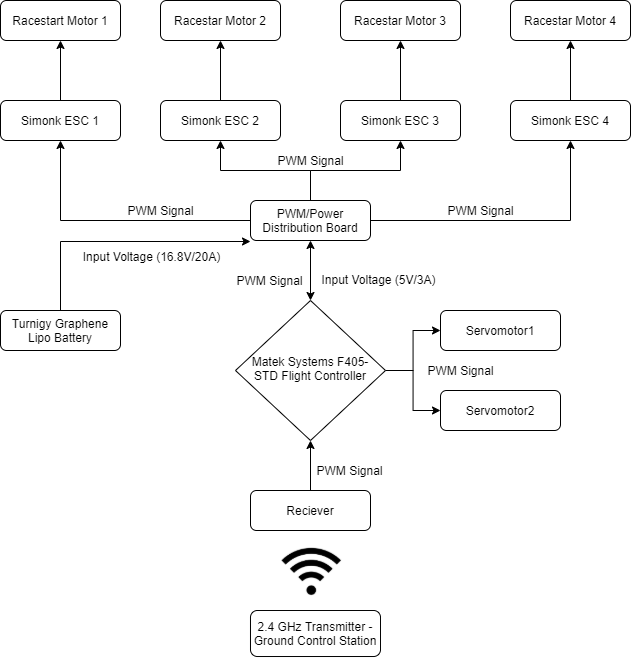
\includegraphics[width=\textwidth]{powerElectronics/systemarchitecture.png}
    \caption{Power Electronics Integration Flow Diagram}
    \label{fig:powerElectronicsFlow}
\end{figure}
\clearpage

\subsubsection{Summary}
This section has outlined a full set of components such that a minimum complexity VTOL system can be constructed. While this system will not provide meaningful data for analysis of mechanism and power requirements, it will provide imperative feedback regarding control complexity and feasibility.
\subsubsection{Future Work}
This minimum complexity system will provide an initial understanding of level of control achievable through commercially available power electronics. Further development requires deeper analysis into specific performance and power requirements as a result of preliminary sizing values concluded in Table~\ref{tab:preresults}. Servomotor requirements will need further analysis of the tilt-wing mechanism to discover expected forces experienced by the mechanism throughout flight. Results from such analysis will heavily impact the style of servomotor selected in the final manufactured prototype. Control link requirements will be further refined once the number of required control inputs and level of autonomy is confirmed.